
The approaches presented herein are inspired by Johansen\cite{mcnotes}.



Let $\chain$ be the chain under consideration, $X_i \sim \dist$ with $\dist$ some distribution and $\phi : \R \rightarrow \R$ be a function. 

$\phi$ is used to estimate key quantities describing $\dist$ by evaluating $\int \phi(x) \, dP(x)$\footnote{whenever this term exists and is well-defined}; setting $\phi = id$ yields the mean and $\phi(x) := x^2$ can then be used to estimate the variance. 

 
With this setup, there are several aspects of convergence to consider: 
\begin{itemize}
	\item whether the chain has reached a stationary regime
	\item whether the chain explores the full support of the target distribution 
	\item the independence of the chain's elements 
\end{itemize}

In the following, we will not address the second aspect.
This is because the distribution we are sampling from is a posterior distribution, whose closed form is unavailable to us. Hence, there is no straightforward way to define the support we expect the distribution to have.

Often, convergence of the chain is confirmed by visual inspection. However, we are interested in developing measures which can be used automatically (i.e. without human intervention) to ascertain convergence. Those methods will come in handy when evaluating how the algorithms' performance depends on the dimension of the problem.

\subsection{Stationarity}
\label{chap:stationarity}
Let 
\[
	\edf{x} := \frac{\sum\limits_{i=1}^T 1_{X_i \leq x}}{T}
\]
This is called the \textit{empirical distribution function}, computed based on the first $T$ elements of the chain.
The indicator functions $1_{X_i \leq x}$ each assume $1$ if $X_i \leq x$ and $0$ otherwise \footnote{Even though it is referred to as a \textit{function}, it depends, in fact, on the underlying $\omega \in \Omega$ of the probability space and is hence actually a so-called \textit{sample function}. }. 

By the \textit{Glivenko-Cantelli theorem}, we have
\[
	\norm{\hat{F}_n - F}_\infty \overset{a.s.}{\longrightarrow} 0
\]

Once the chain has reached its stationary regime, we expect the empirical distribution function to have converged as well. Hence, we can use differences between empirical distribution functions of the chain at different points in time to measure convergence to stationarity. We adopt an idea originally presented by Dr. Pieralberto Guarniero in a practical seminar in the context of Riemann sums: 
The chain of length $T$ is split into three components of equal size $s := \floor{\frac{T}{3}}$: 
\[
S_1 := \left(X_1, \dots, X_s\right), S_2 := \left(X_s, \dots, X_{2s}\right), S_3 := \left(X_{2s}, \dots, X_T\right)
\] 

Figure \ref{splitChain} illustrates how the chain is split. Note that in the first part, the parameters are still diverging from their initial values; this part is referred to as  ''burn-in period''. Note that because the way from the initial estimates is included, this part's empirical distribution function is usually far from the desired distribution. Therefore, the very first part is usually ignored in this analysis.

Upon a brief, graphical inspection, one might conclude that the second and third part's distribution seems to be equal and in particular, that the distribution reached stationarity after about $50$ samples.  


Figure \ref{splitChainDensities} shows the estimated densities\footnote{as they are graphically easier to understand than the estimated empirical distribution function itself; the densities are estimated using ''geom\_density'' from ggplot2 with Gaussian smoothing (n=128, adjust = 0.25)} for all three parts of the chain; one can clearly see that the second and third chains' modes are already ''zeroing in'' on the original probability (which is $0.9$), while the first density is still highly skewed towards the initial choice. 

Note how the second chain's density still exhibits multiple modes, whereas the third chain only has one main mode left (which is incidentally closer to the original value). Visual inspection of the chain itself fails to reveal this, making it a prime example of how an quantitative analysis can outdo mere visual inspection of the chain. However, the median (indicated by a green line) is the same for the second and third part. 


\begin{figure}
	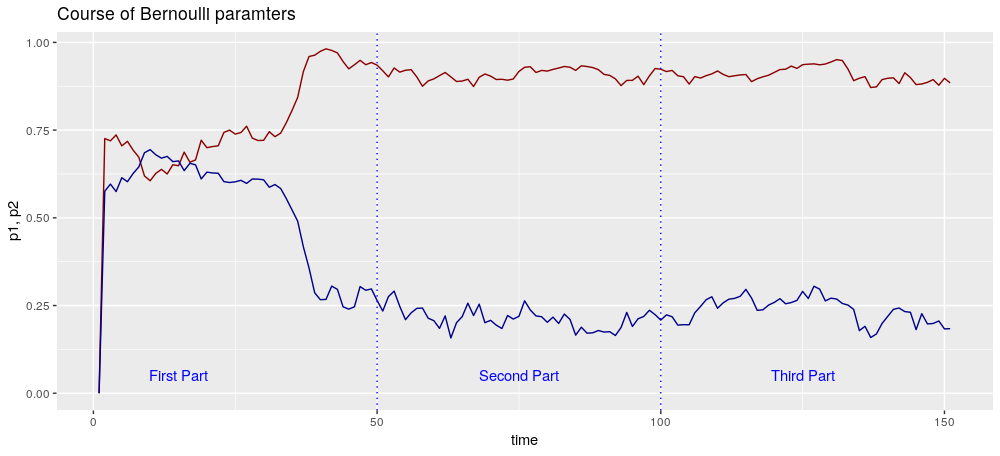
\includegraphics[width=\linewidth]{Images/bernoulli_param_split.png}
	\caption{Course of Bernoulli parameters for Gibb's sampler on simple rain model}
	\label{splitChain}
\end{figure}

\begin{figure}
	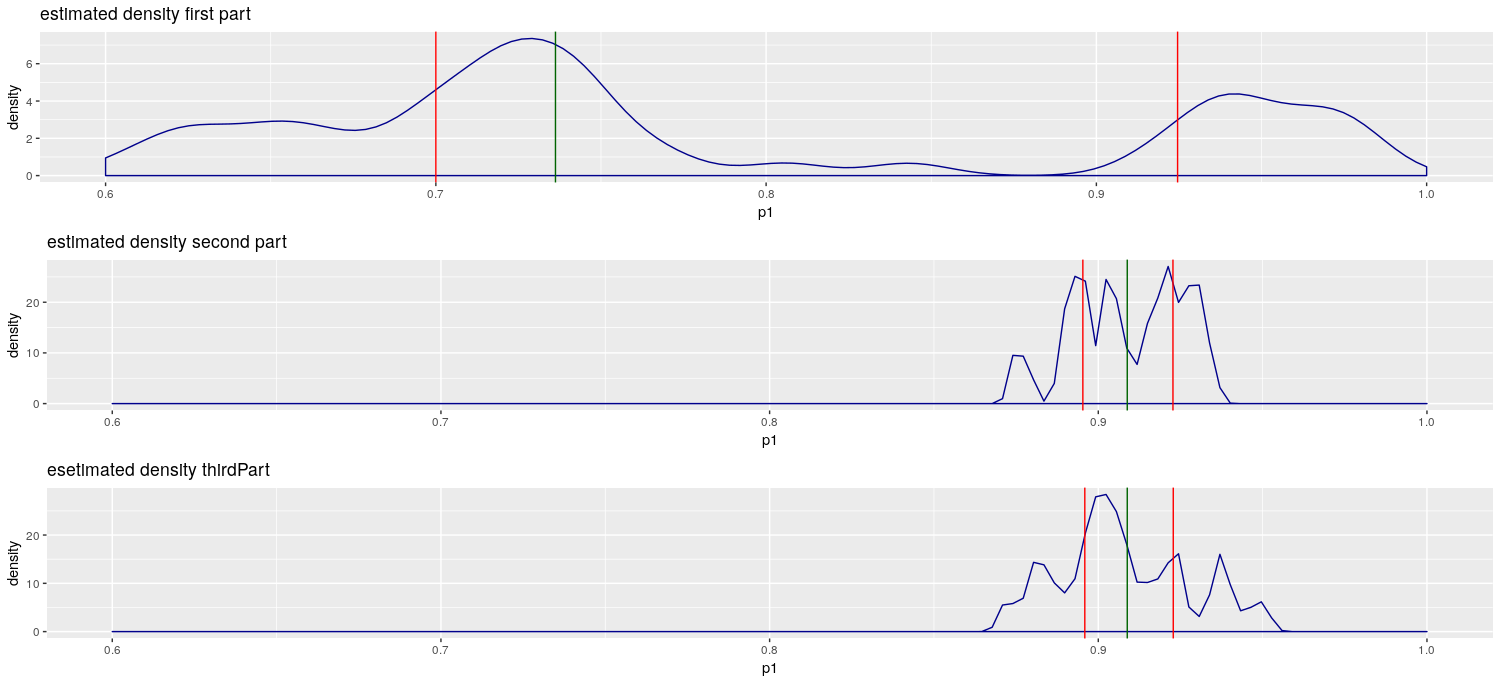
\includegraphics[width=\linewidth]{Images/chain_parts_quantiles.png}
	\caption{Density estimates for $S_1, S_2$ and $S_3$ with $0.25, 0.5$ and $ 0.75$ quantiles (red, green, red) indicated by lines}
	\label{splitChainDensities}
\end{figure}

Figure \ref{splitChainQuantileCourse} allows us to quantitatively confirm the results from the visual inspection. We observe:
\begin{itemize}
	\item the third part reaches its stationary regime earlier than the second part
	\item the second part's quantiles converge toward the third part's quantiles
\end{itemize}

Note that the second and third parts' quantiles in figure \ref{splitChainQuantileCourse} become visually indistinguishable after a sample size of about $120$. 

At this point, the maximum difference has fallen below $0.01 (1\%)$. 
Also, the second part comprises elements from about $X_{40}, \dots, X_{80}$ whereas the third part comprises $X_{80}, \dots, X_{120}$. This is consistent with our intuitive conclusion from figure \ref{splitChain} that the chain reaches its stationary regime after about $50$ samples. 

\begin{figure}
	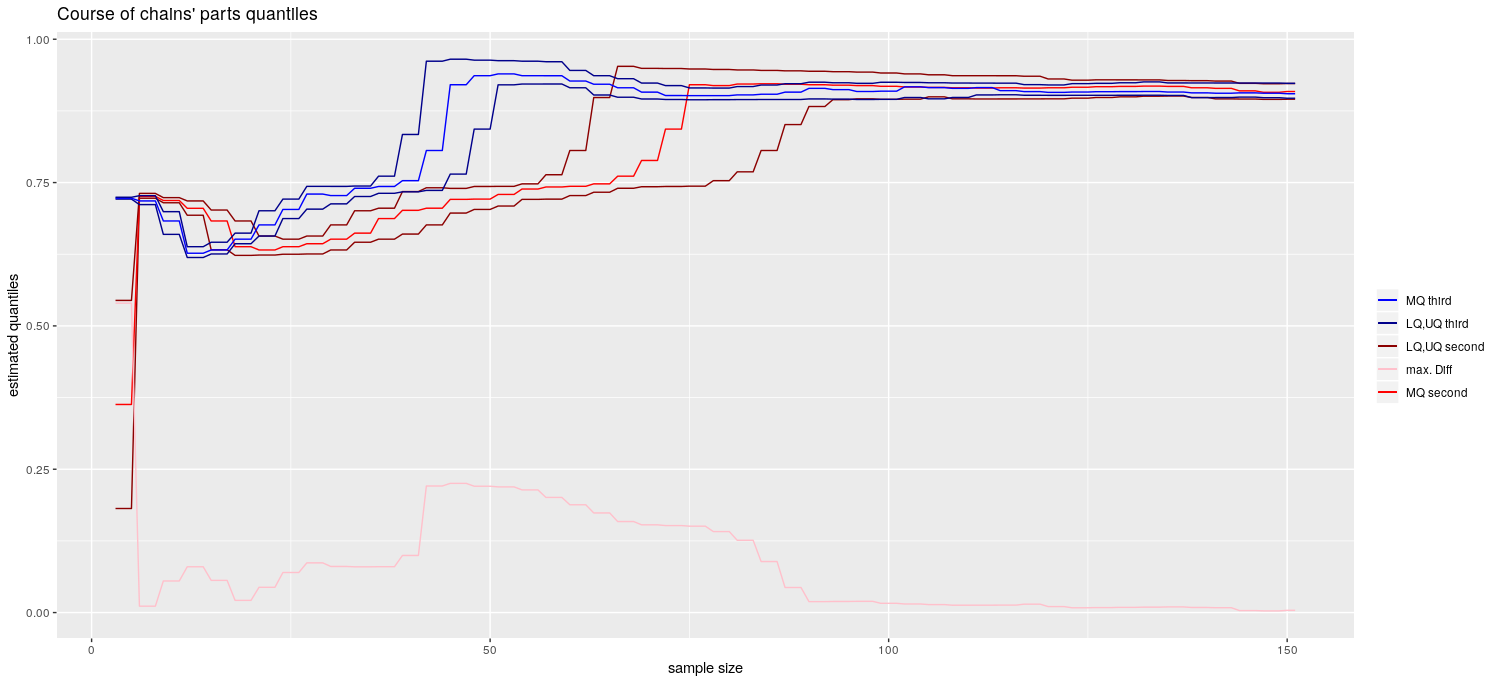
\includegraphics[width=\linewidth]{Images/chain_part_quantiles.png}
	\caption{Course of quantiles for the second and third part of the chain. ''LQ, MQ and UP'' are shortcuts for ''lower'', ''middle'' and ''upper' quantile and refer to the $0.25, 0.5$ and $0.75$ quantiles, respectively. ''second'' and ''third' refer to which part of the chain is considered for computing the quantiles. ''Max. Diff'' (pink) denotes the maximum difference between respective quantiles at each point in time. }
	\label{splitChainQuantileCourse}
\end{figure}

\subsubsection*{Insignificance of $\delta$}
Also note that for large sample sizes, the choice of $\delta$ usually becomes irrelevant. This is because compared to the overall length of the chain, the contribution of $\delta$ tends towards insignificance. For this reason, $\delta$ is hardly estimable, i.e. we expect great fluctuation in its quantiles. Hence, for convergence analysis, $\delta$ is discarded. 
\vspace{0.5cm}

In conclusion, we have developed a quantitative measure for stationarity of the chain's distribution. 
We shall adopt the criterion developed herein with a cut-off criterion of $0.01$. In our experiments, a convergence up to said threshold usually implied a good conversion of the overall sampling distribution.
 That is to say: 

\begin{center}
We assume that the chain has reached convergence once the maximum difference between the $0.25, 0.5$ and $0.75$ quantiles of the second and third part are smaller than $0.01$. 
\end{center}


\subsection{Independence of Elements}

Independence of the elements is also crucial to the quality of the chain's approximation. The more consecutive samples depend on each other, the lower the amount of information for inferential purposes is. 

For instance, when estimating the variance, if the samples $\chain$ are \textit{not independent}, then the estimate of the variance of $\phi(X_t)$ is 
\[
Var \left(	\frac{1}{T} \, \sum\limits_{t=1}^T \phi(X_t)\right)
\]
 This will typically be greater than the variance of i.i.d. samples, which is $\frac{Var\left(\phi(X_t) \right)}{T}$. 

The effective sample size (ESS) quantifies statistical dependence by computing the number of samples $\chain$ which would yield the same variance as if i.i.d. samples were used. 

For illustrative purposes, we follow the methodology presented in Johansen \cite{mcnotes}; in practice, more sophisticated solutions would be in order. 

Assume that $\chain$ is a second-order stationary time series, that is $Var \left( \phi(X_t)	\right) = \sigma^2$ and $p(X_t, X_{t+\tau}) = p(\tau)$ for $\forall t, \tau \in \nn$ and $p(\tau)$ is the \textit{correlation} at lag $\tau$. 

Then, Johansen \cite{mcnotes} shows that:
\begin{align*}
	T \,  Var\left( 
		\frac{1}{T} \, \sum\limits_{i=1}^T \phi(X_t) 
	\right)
	\overset{T \rightarrow \infty}{\longrightarrow} 
	\sigma^2 \left(
		1 + 2 \sum\limits_{i=1}^\infty p(\tau)
	\right)
\end{align*}

For i.i.d. samples we have 
\begin{align*}
	 Var\left( 
	\frac{1}{T_{\text{ess}}} \, \sum\limits_{i=1}^T \phi(X_t) 
	\right) = \frac{\sigma^2}{T_{\text{ess}}}
\end{align*}

Equating both evaluations yields
\[
	T_{\text{ess}} = \frac{1}{	1 + 2 \sum\limits_{i=1}^\infty p(\tau)} \, T
\]

As the correlations can be computed empirically, this gives us an estimate of the ESS. 


\subsection{Hidden States}
One of the algorithms under scrutiny, namely the Gibb's sampler, estimates the hidden states explicitly. Hence, this estimate can be used to ascertain whether the chain has converged towards its stationary distribution as well.

There are two things to note here:
\begin{itemize}
\item  this comparison will not be meaningful depending on the system in question. \\
 If the states do not differ significantly, they are hardly estimable by only considering the observations.
\item when applying the algorithms to real data, the hidden states are usually not available. Hence, this measure is only used to confirm the viability of solutions found for synthetic data. In this respect, it backs up the measures defined earlier. 
\end{itemize}


Note that the algorithm's hidden states samples generally will not and should not equal the states used when originally sampling the observations. This is for the simple reason that the observations are not drawn according to the maximum likelihood.

 For each state, we draw from the state's distribution; thus we will not just draw the value which is most likely to be drawn. This way, the overall likelihood is also less than the maximum likelihood. The hidden states' estimate will have a lower likelihood than the MLE solution. 

However, there is an (analytical) way to compute the \textit{expected deviation} from the original chain of hidden states. 
To this end, let us consider the $L_1(\R^T)$\footnote{$\norm{x} := \sum |x|$} distance between the original chain $\left(C_1, \dots, C_T\right)$ and the sampled chain $\left(\tilde{C}_1, \dots \tilde{C}_T\right)$. 

We expect $P(C_t = i)$ to be high (i.e. $i$ likely to be sampled as the hidden state at time $t$) iff $\prob{X_t = x_t}{ C_t = i}$ is high. Let $j := \text{maxarg} \prob{X_t = x_t}{C_t = j}$. Then we expect to misestimate the state with a probability of $\omega := \sum\limits_{i = 1, i \neq j}^T \prob{X_t = x_t}{C_t = i}$. 

Furthermore, once the chain as reached stationarity, this allows us to compute the expected number of deviated states: it is $ T * \omega$. 

\begin{figure}
	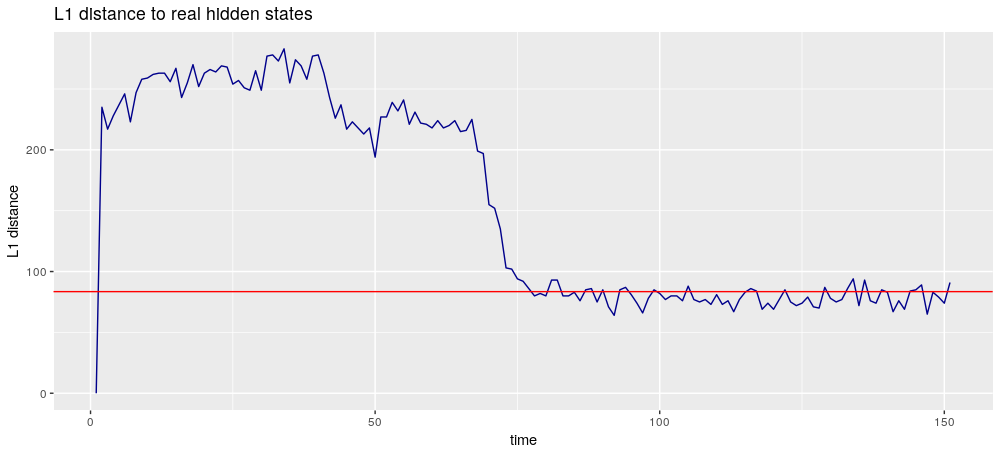
\includegraphics[width=\linewidth]{./img/l1_hidden_state_distance.png}
	\caption{The red line indicates the expected number of wrong hidden states, the blue number the number of wrong hidden states at points $t$ of the sampled chain. We clearly see that after about $70$ iterations, the algorithm has reached the expected value. }
	\label{l1_wrong_states}
\end{figure}









